%!TEX root = guided_inpainting_paper.tex
\section{Our Method}

\begin{figure*}[ht!]
\centering
\small
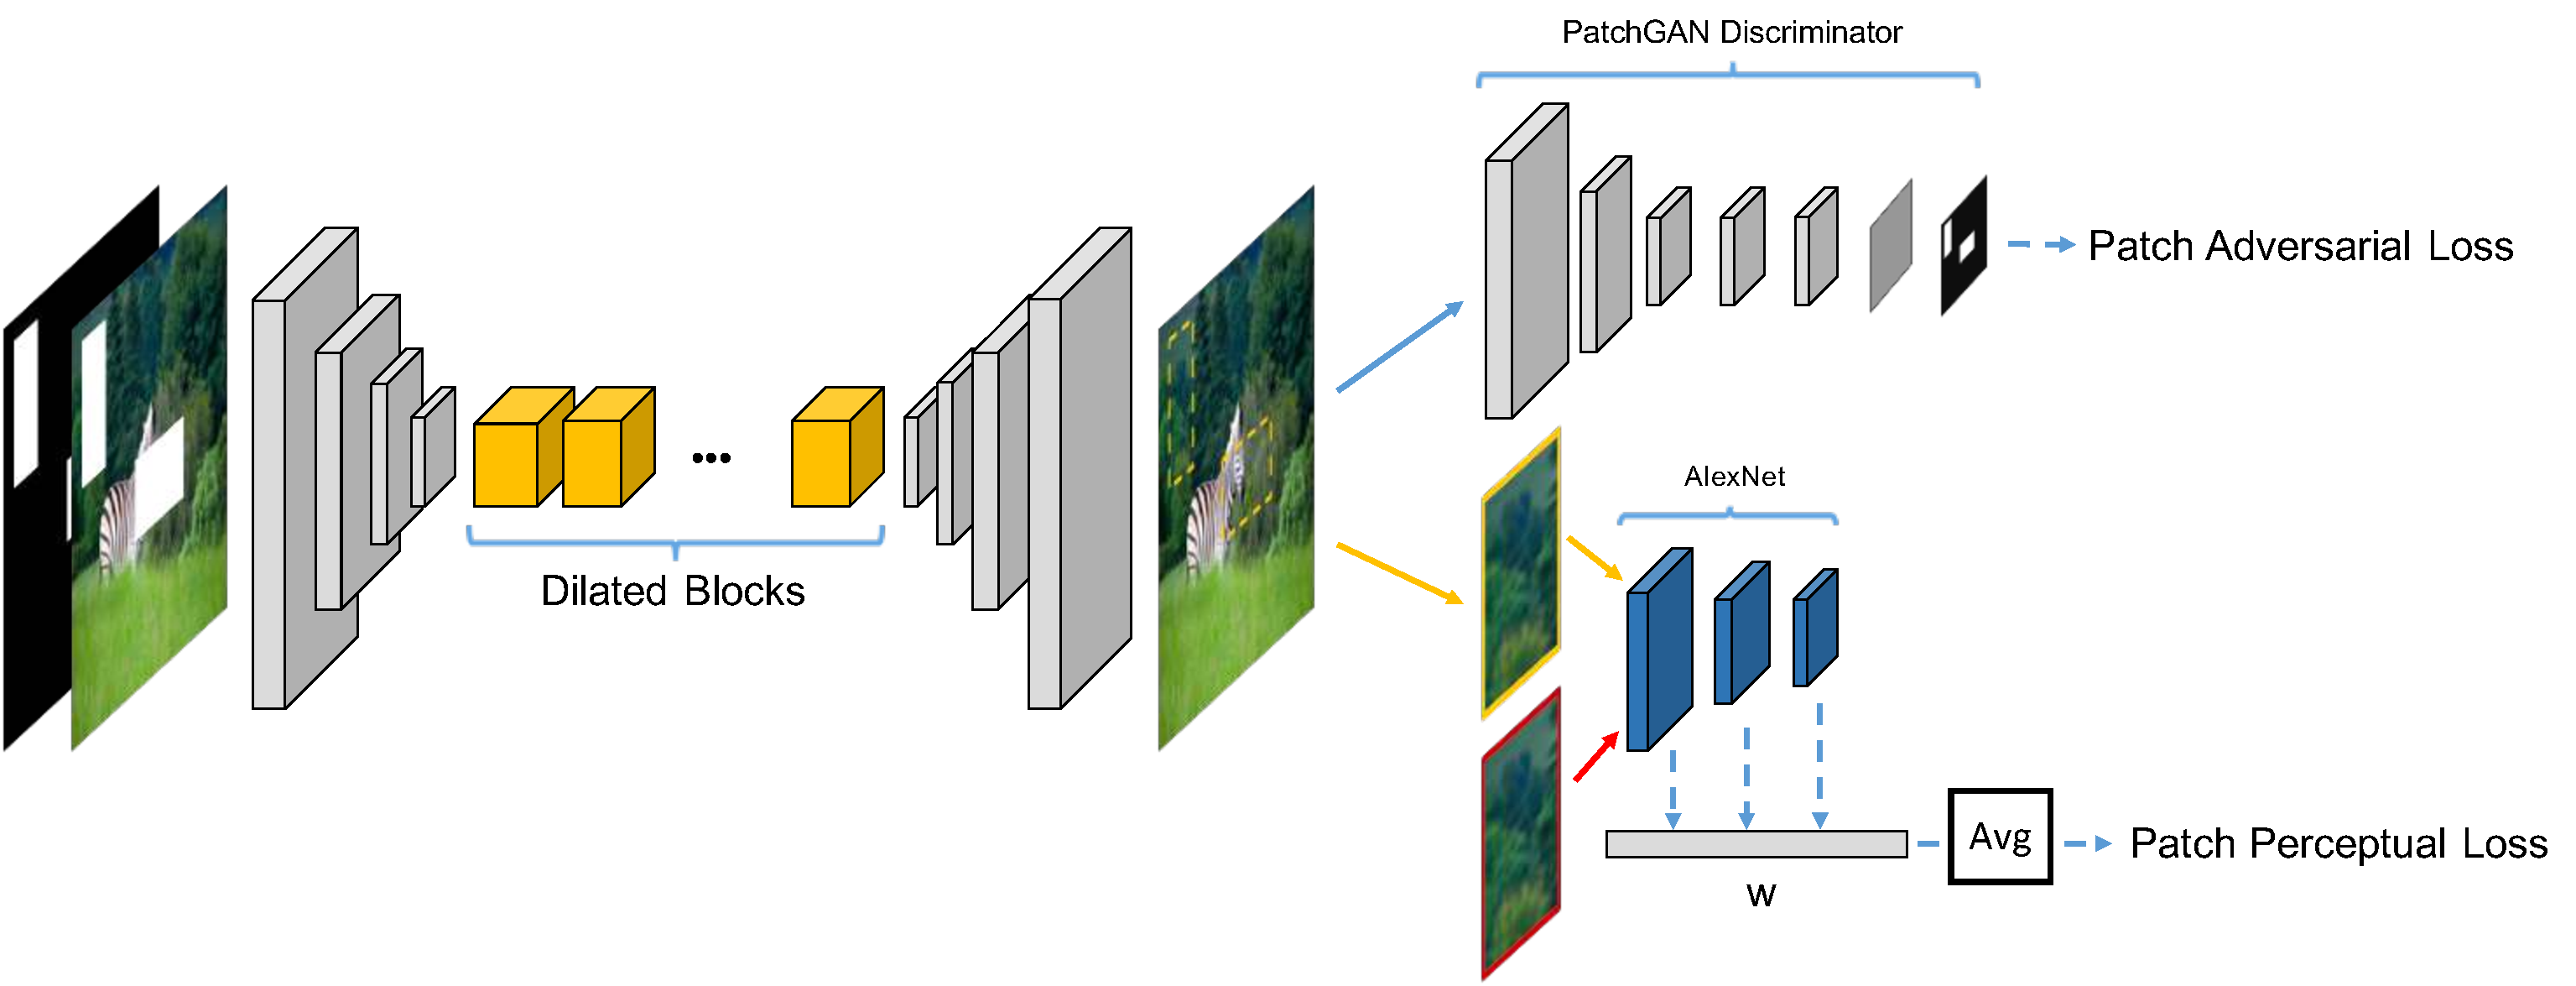
\includegraphics[width=1\textwidth]{figures/arch2.pdf}
\caption{Generator head and the training losses. We only illustrate one scale of Patch Adversarial Loss and Patch Perceptual Loss. Note that to compute the Patch Adversarial Loss, we need to use the mask to find out which patch overlaps with the hole.}
\label{fig:model}
\vspace{-15pt}
\end{figure*}

Our method consists of training a generator head as initialization and optimizing additional residual blocks as refinement. The generator head is trained for inpainting and is based on conditional GAN framework. Vanilla cGAN for image inpainting consists of a Generator $G$ and a Discriminator $D$. The generator learns to predict the hole contents and restore the complete image, while the discriminator learns to distinguish real images from generated images. Using the original image as ground truth, the model is trained in a self-supervised manner via the following minimax objective:
\begin{eqnarray}
\min\limits_G \max\limits_D E_{(s,x)}[\log D(s,x)] + E_s[\log (1-D(s,G(s)))].
\end{eqnarray}
Here $s$ and $x$ are the incomplete image as input and the original image as target. $G(s)$ is the output of the generator which could be the hole content or the complete image. In the case when $G(s)$ restores the complete image, only the contents inside the hole are kept to combine with the known regions of $s$.

\subsection{The Generator Head}
\label{sec:resnet_head}

Existing works have investigated different architectures of $G$, most notably the encoder-decoder style of~\cite{pathak2016context} and the FCN style of~\cite{iizuka2017globally}. ~\cite{iizuka2017globally} shows that FCN generates higher-quality and less blurred results comparing with encoder-decoder, largely because the network used is much deeper and is fully convolutional. In contrast, the encoder-decoder in~\cite{pathak2016context} uses an intermediate bottleneck, fully-connected layer, which results in size reduction and information loss. 

Similar to~\cite{iizuka2017globally}, our generator head is based on FCN and leverage the many properties of convolutional neural networks, such as translation invariance and parameter sharing. However, a major limitation of FCN is the constraint of the receptive field size. Given the convolution layers are locally connected, pixels far away from the hole carry no influence on the hole. We propose several modifications to alleviate this drawback. First, we build our network with three components: a down-sampling front end to reduce the size, followed by multiple residual blocks~\cite{he2016deep}, and an up-sampling back end to restore the full dimension. Using down-sampling increases the receptive field of the residual blocks and makes it easier to learn the transformation at a smaller size. Second, we stack multiple residual blocks to further enlarge the view at later layers. Finally, we adopt the dilated convolution~\cite{yu2015multi} in all residual blocks, with the dilation factor set to 2. Dilated convolutions use spaced kernels, making it compute each output value with a wider view of input without increasing the number of parameters and computational burden. From experiments, we observe that increasing the size of the receptive field, especially by using dilated convolution, is critical for enhanced inpainting quality. In contrast, other image translation tasks such as super-resolution, denoising, etc., usually rely more on local statistics rather than global context.

The detail of our architecture is as follows: the down-sampling front end consists of three convolutional layers, each with a stride of 2. The intermediate part contains 9 residual blocks, and the up-sampling back-end consists of three transposed convolution, also with a stride of 2. Each convolutional layer is followed by batch normalization (BN) and ReLu activation, except for the last layer which outputs the image. Similar architecture without dilated convolution has been used in~\cite{wang2017high} for image synthesis. Comparing with~\cite{iizuka2017globally}, our receptive field is much larger, as we adopted more down-sampling and dilated layers. This makes us generate better results with less artifacts. As ablation study, we compare different types of layers and architectures in Sec.~\ref{exp:study}.

\subsection{The Training Losses}
Different losses have been used to train an inpainting network. These losses can be cast into two categories. The first category which can be referred to as \textit{similarity loss}, is used to measure the similarity between the output and the original image. The second category which we refer to as the \textit{realism loss}, is used to measure how realistic-looking is the output image. We summarize the losses used in different inpainting methods in Table~\ref{table:losses}. 

\begin{table}[h!]
\begin{center}
\resizebox{.5\textwidth}{!}{%
{\tiny
  \begin{tabular}{ l  c  c }
    \hline
    \textbf{Method} & \textbf{Similarity Loss} &  \textbf{Realism Loss} \\ \hline
    \emph{CE~\cite{pathak2016context}} & $\ell_2$ & Global Adversarial Loss\\ \hline
    \emph{GLI~\cite{iizuka2017globally}} & $\ell_2$ & Global and Local Adversarial Loss \\ \hline
    \emph{Ours} & Patch Perceptual Loss & Multi-Scale Patch Adversarial Loss \\ \hline
    \hline
  \end{tabular}}
  }
  \end{center}
  \caption{Comparison of training losses used in different methods.}
  \label{table:losses}
\end{table}

\noindent\textbf{Patch Perceptual Loss} As shown in Table~\ref{table:losses}, using $\ell_2$ as reconstruction loss to measure the difference between the output and the original image has been the default choice of previous inpainting methods. However, it is known that $\ell_2$ loss does not correspond well to human perception of visual similarity (Zhang et al.~\cite{zhang2018unreasonable}). This is because using $\ell_2$ assumes each output pixel is conditionally independent of all others, which is not the case. An example is that blurring an image leads to small changes in terms of $\ell_2$ distance but causes significant perceptual difference. Recent research suggests that a better metric for perceptual similarity is the internal activations of deep convolutional networks, usually trained on a high-level image classification task. Such loss is called ``perceptual loss'', and is used in various tasks such as neural style transfer~\cite{gatys2016image}, image super-resolution~\cite{johnson2016perceptual}, and conditional image synthesis~\cite{dosovitskiy2016generating,chen2017photographic}.

Based on this observation, we propose a new ``patch perceptual loss'' as the substitute of the $\ell_2$ losses. Traditional perceptual loss typically uses VGG-Net and computes the $\ell_2$ distance of the activations on a few feature layers. Recently,~\cite{zhang2018unreasonable} trained a specific perceptual network based on AlexNet to measure the perceptual differences between two image patches, making it an ideal candidate for our task. The perceptual network computes the activations and sums up the $\ell_2$ distances across all feature layers, each scaled by a learned weight. Furthermore, taking both the local view and the global view into account, we compute PPL at two scales. Local PPL considers the local hole patch, while the global PPL slightly zooms out to cover a larger contextual area. More formally, our PPL is defined as:
\begin{eqnarray}
&& \sum\limits_{p=p_1,p_2}PPL(G(s)_p, x_p) \\ \nonumber
&&= \sum\limits_{p=p_1,p_2}\sum\limits_l\frac{1}{H_lW_l}\sum\limits_{h,w}\parallel w_l^T\odot(\hat{F}(x_p)^l_{hw}-\hat{F}(G(s)_p)^l_{hw})\parallel^2_2.
\end{eqnarray}

Here $p$ refers to the hole patch. $\hat{F}$ is the AlexNet and $l$ is the feature layer. $w_l$ is the layer-wise learned weight. Ablation study in Sec.~\ref{exp:study} shows that our patch perceptual loss gives better inpainting quality than traditional $\ell_2$. 

\noindent\textbf{Multi-Scale Patch Adversarial Loss} Adversarial losses are given by trained discriminators to discern whether an image is real or fake. The global adversarial loss of~\cite{pathak2016context} takes the entire image as input and outputs a single real/fake prediction which does not consider local realism of holes. The additional local adversarial loss of~\cite{iizuka2017globally} adds another discriminator specifically for the hole, but it requires the hole to be fixed in shape and size during training to fit the local discriminator. To consider both the global view and the local view, and to be able to use multiple holes of arbitrary shape, we propose to use PatchGAN discriminators~\cite{isola2016image} at three scales of image resolutions. The discriminator at each scale is identical and only the input is a differently scaled version of the \textit{entire image}. Each discriminator is a fully convolutional PatchGAN and outputs a vector of real/fake predictions and each value corresponds to a local image patch. In this way, the discriminators are trained to classify global and local patches across the image at multiple scales, and it enables us to use multiple holes of arbitrary shapes since now the input is the entire image rather than the hole itself. However, since the output image is the composition of synthesized holes and known background, directly using PatchGAN is problematic because it does not differentiate between the hole patches (\textit{fake}) and the background patches (\textit{real}). To address this issue, when computing the PatchGAN loss, only the patches that overlap with the holes are labeled as fake. More formally, our Patch-wise Adversarial Loss is defined as: 
\begin{eqnarray}
&&\min\limits_G\max\limits_{D_1, D_2, D_3}\sum\limits_{k=1,2,3} L_{GAN}(G,D_k)  \\ \nonumber
&&=\sum\limits_{k=1,2,3}E_{(s_k,x_k)}[\log (s_k,x_k)] + E_{s_k}[\log (Q_k-D_k(s_k,G(s_k)))].
\end{eqnarray}
\label{eqn:adversarial_loss}
Here $k$ refers to the image scale, and $Q_k$ is a patch-wise real/fake vector, based on whether the patch overlaps with the holes. Using multiple GAN discriminators at the same or different image scale has been proposed in unconditional GANs~\cite{durugkar2016generative} and conditional GANs~\cite{wang2017high}. Here we extend the design to take into account the holes, which is critical for obtaining semantically and locally coherent image completion results.

To summarize, our full objective combines both losses is therefore defined as:

\begin{eqnarray}
\min\limits_G((\max\limits_{D_1, D_2, D_3}\lambda_{Adv}\sum\limits_{k=1,2,3} L_{GAN}(G,D_k)) \\ \nonumber
+\lambda_{PPL}\sum\limits_{k=1,2}PPL_k(G(s)_p, x_p)).
\end{eqnarray}

We use $\lambda_{Adv}$ and $\lambda_{PPL}$ to control the importance of the two terms. In our experiment, we set initial $\lambda_{Adv}=1$ and $\lambda_{PPL}=10$ as used in~\cite{pathak2016context,wang2017high}. As training progresses, we gradually decrease the weight of $\lambda_{Adv}$ based on adversarial loss annealing (Sec.~\ref{sec:procedural}).

Fig.~\ref{fig:model} illustrates the architecture of our generator head and the training losses.

\subsection{Blockwise Procedural Training with Adversarial Loss Annealing}
\label{sec:procedural}
Our experiments show that using the described generator head and training losses already generate results of descent quality. An intuitive effort to improve the results would be to stack more intermediate residual blocks to further expand the receptive view and increase the expressiveness of the model. However, we found that directly stacking more residual blocks makes it more difficult to stabilize the training. As the parameter space becomes much larger, it is also more challenging to find local optimum. In the end, the inpainting quality deteriorates as the model depth increases.

\begin{figure}[t]
\centering
\small
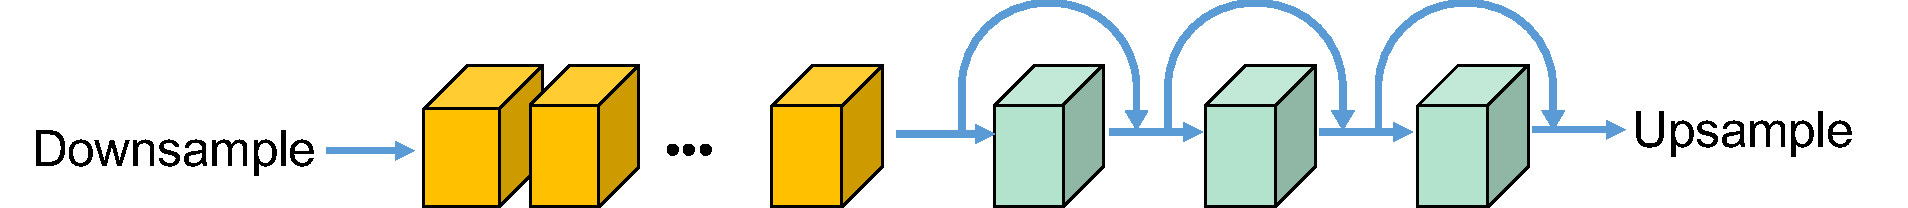
\includegraphics[width=.45\textwidth]{figures/proc.pdf}
\caption{Illustration of block-wise procedural training. The yellow residual blocks refer to the generator head which is trained first. The green residual blocks are progressively added one at a time. We also draw the skip connections between the already trained residual blocks and the up-sampling back end.}
\label{fig:procedural}

\end{figure}

To address the challenge of training a deeper network, we propose to use procedural block-wise training to gradually increase the depth of the inpainting network. More specifically, we begin by training the generator head until it converges. Then, we add a new residual block after the already trained residual blocks, right before the back-end up-sampling layers. In order to smoothly introduce the new residual block without breaking the trained model, we add another skip path from the already trained residual blocks to the up-sampling layers. Initially, the weight of the skip path is set to 1, while the weight of the path containing the new block is set to 0. This essentially makes the initial network identical to the already trained network. We then slowly decrease the weight of the skip path and increase the weight of the new residual block as training progresses. In this way, the newly introduced residual block is trained to be a fine-tuning component, which adds another layer of fine details to the original results. This step are repeated multiple times, and each time we deepen the network by adding a new residual block. In our experiments, we found that the results improve significantly over generator head, after training with the first residual block added. The output becomes stabilized after three residual blocks, and very little changes can be detected if more residual blocks are brought in. We illustrate the procedural training process in Fig.~\ref{fig:procedural}.

The block-wise procedural training has several benefits. First, it guides the training process of a very deep generator. Starting with the generator head and gradually fine-tuning with more residual blocks makes it easier to discover the mapping between the incomplete image and the complete image, even though the search space is huge given the diversity of natural images and the randomness of holes. Another benefit is training efficiency, as we found decoupling the training of the generator head and the fine-tuning of additional residual blocks requires significantly less training time comparing with training the network all at once. Similar idea of progressive training has been used in Progressive GAN~\cite{karras2017progressive}. However the task and the model are different in our case.

\noindent\textbf{Adversarial Loss Annealing} During training, the generator adversarial loss updates the generator weight if the discriminator successfully detects the generated image as fake:
\begin{eqnarray}
\sum\limits_{k=1,2,3}E_s[\log (\bar{Q}-D_k(s_k,G(s_k)))].
\end{eqnarray}
Note that here $\bar{Q}$ reverses $Q$ of~\ref{eqn:adversarial_loss} as this is the loss to the generator. We observe that the generator adversarial loss becomes dominant over PPL as training progresses, as the discriminator becomes increasingly good at detecting fake images during training. This is less of a problem for image synthesis tasks. However, for the inpainting task which requires the output to be faithful to the original image, the outcome is that the generator deliberately adds noise patterns to confuse the discriminators, leading to artifacts or incorrect textures. Based on this observation, we propose to use adversarial loss annealing, which decreases the weight of the adversarial loss for the generator at the time of adding new residual blocks. More formally, let the initial weight of the generator adversarial loss be $\lambda^0_{adv}$, and the weight of the generator adversarial loss be $\lambda^i_{adv}$ after adding the $i_{th}$ residual block. We found that simply decay the weight linearly by setting $\lambda^i_{G_{adv}}=10^{-i}\lambda^0_{G_{adv}}$ gives results significantly better than using constant weight. In Sec.~\ref{sec:results}, we analyze the effect of ALA in more detail.

Finally, we summarize the discussed training schemes in Alg.~\ref{algo}.
\begin{algorithm}
\caption{Training the Inpainting Network}\label{algo}
\begin{algorithmic}[1]
\State Set batch size to 8 and basic learning rate to $lr_0\gets 0.0002$.
\State Set $\lambda_{PPL}\gets 10$ and $\lambda^0_{{adv}}\gets 1$.
\State Train the Generator Head $G_0$ using MSPAL and PPL (\ref{eqn:adversarial_loss}) for 150,000 iterations.
\For{i=1 to 3}
\State Add the skip path and the residual block $r_i$.
\State Set $lr_i\gets 10^{-i} lr_0$ and $\lambda^i_{G_{adv}}\gets 10^{-i}\lambda^0_{G_{adv}}$.
\State Train the generator $G_3$ with the added $r_i$ for 1,500 iterations.
\EndFor
\State \textbf{return} $G_3$ 
\end{algorithmic}
\end{algorithm}
